\documentclass[12pt,a4paper]{article}
\usepackage[margin=1in]{geometry}
\usepackage{booktabs}
\usepackage{threeparttable}
\usepackage{float}
\usepackage{amsmath,amssymb}
\usepackage{graphicx}
\usepackage{caption}
\usepackage[colorlinks=true,linkcolor=blue,citecolor=blue]{hyperref}
\usepackage{setspace}
\onehalfspacing

\title{Bitcoin Halving Event Study:\\
\large Supply Shocks and Market Response}
\author{econtools Research Pipeline}
\date{\today}

\begin{document}
\maketitle

\begin{abstract}
Bitcoin halvings---pre-programmed 50\% reductions in block rewards occurring
approximately every four years---represent exogenous supply shocks of known
timing but uncertain price impact. Using data from 2010--2025 spanning all
four halvings, we conduct an event study analysis combining cumulative
abnormal returns (CARs) with regression-based tests. Wild bootstrap
confidence intervals complement HC3 robust inference.
We find positive but imprecisely estimated post-halving effects on daily
returns, with substantial heterogeneity across halving episodes.
\end{abstract}

\section{Introduction}

Bitcoin's monetary policy is uniquely transparent: the block reward halves
every 210,000 blocks (approximately 4 years), and this schedule has been
known since Bitcoin's inception in 2009. The efficient markets hypothesis
(EMH) predicts that a fully anticipated supply reduction should be priced
in advance. However, if market participants are inattentive or if the
halving triggers narrative-driven demand shifts, post-halving abnormal
returns may persist.

We examine all four Bitcoin halvings (November 2012, July 2016, May 2020,
April 2024) using cumulative log returns in event windows, regime
regressions with robust standard errors, and wild bootstrap inference.

\section{Data and Methodology}

Our dataset covers 5,385 daily observations of Bitcoin prices and
on-chain metrics from CoinMetrics. We define a ``post-halving'' dummy
equal to 1 for the 365 calendar days following each halving event.

We estimate:
\begin{equation}
r_t = \alpha + \beta \cdot \mathbf{1}[\text{Post-Halving}]_t + \gamma' X_t + \varepsilon_t
\end{equation}
where $X_t$ includes lagged volatility, momentum, and on-chain controls.
Standard errors are HC3 heteroskedasticity-robust. We supplement
asymptotic inference with wild bootstrap (Rademacher weights, $B=2{,}000$).

\section{Cumulative Abnormal Returns}

\begin{figure}[H]
\centering
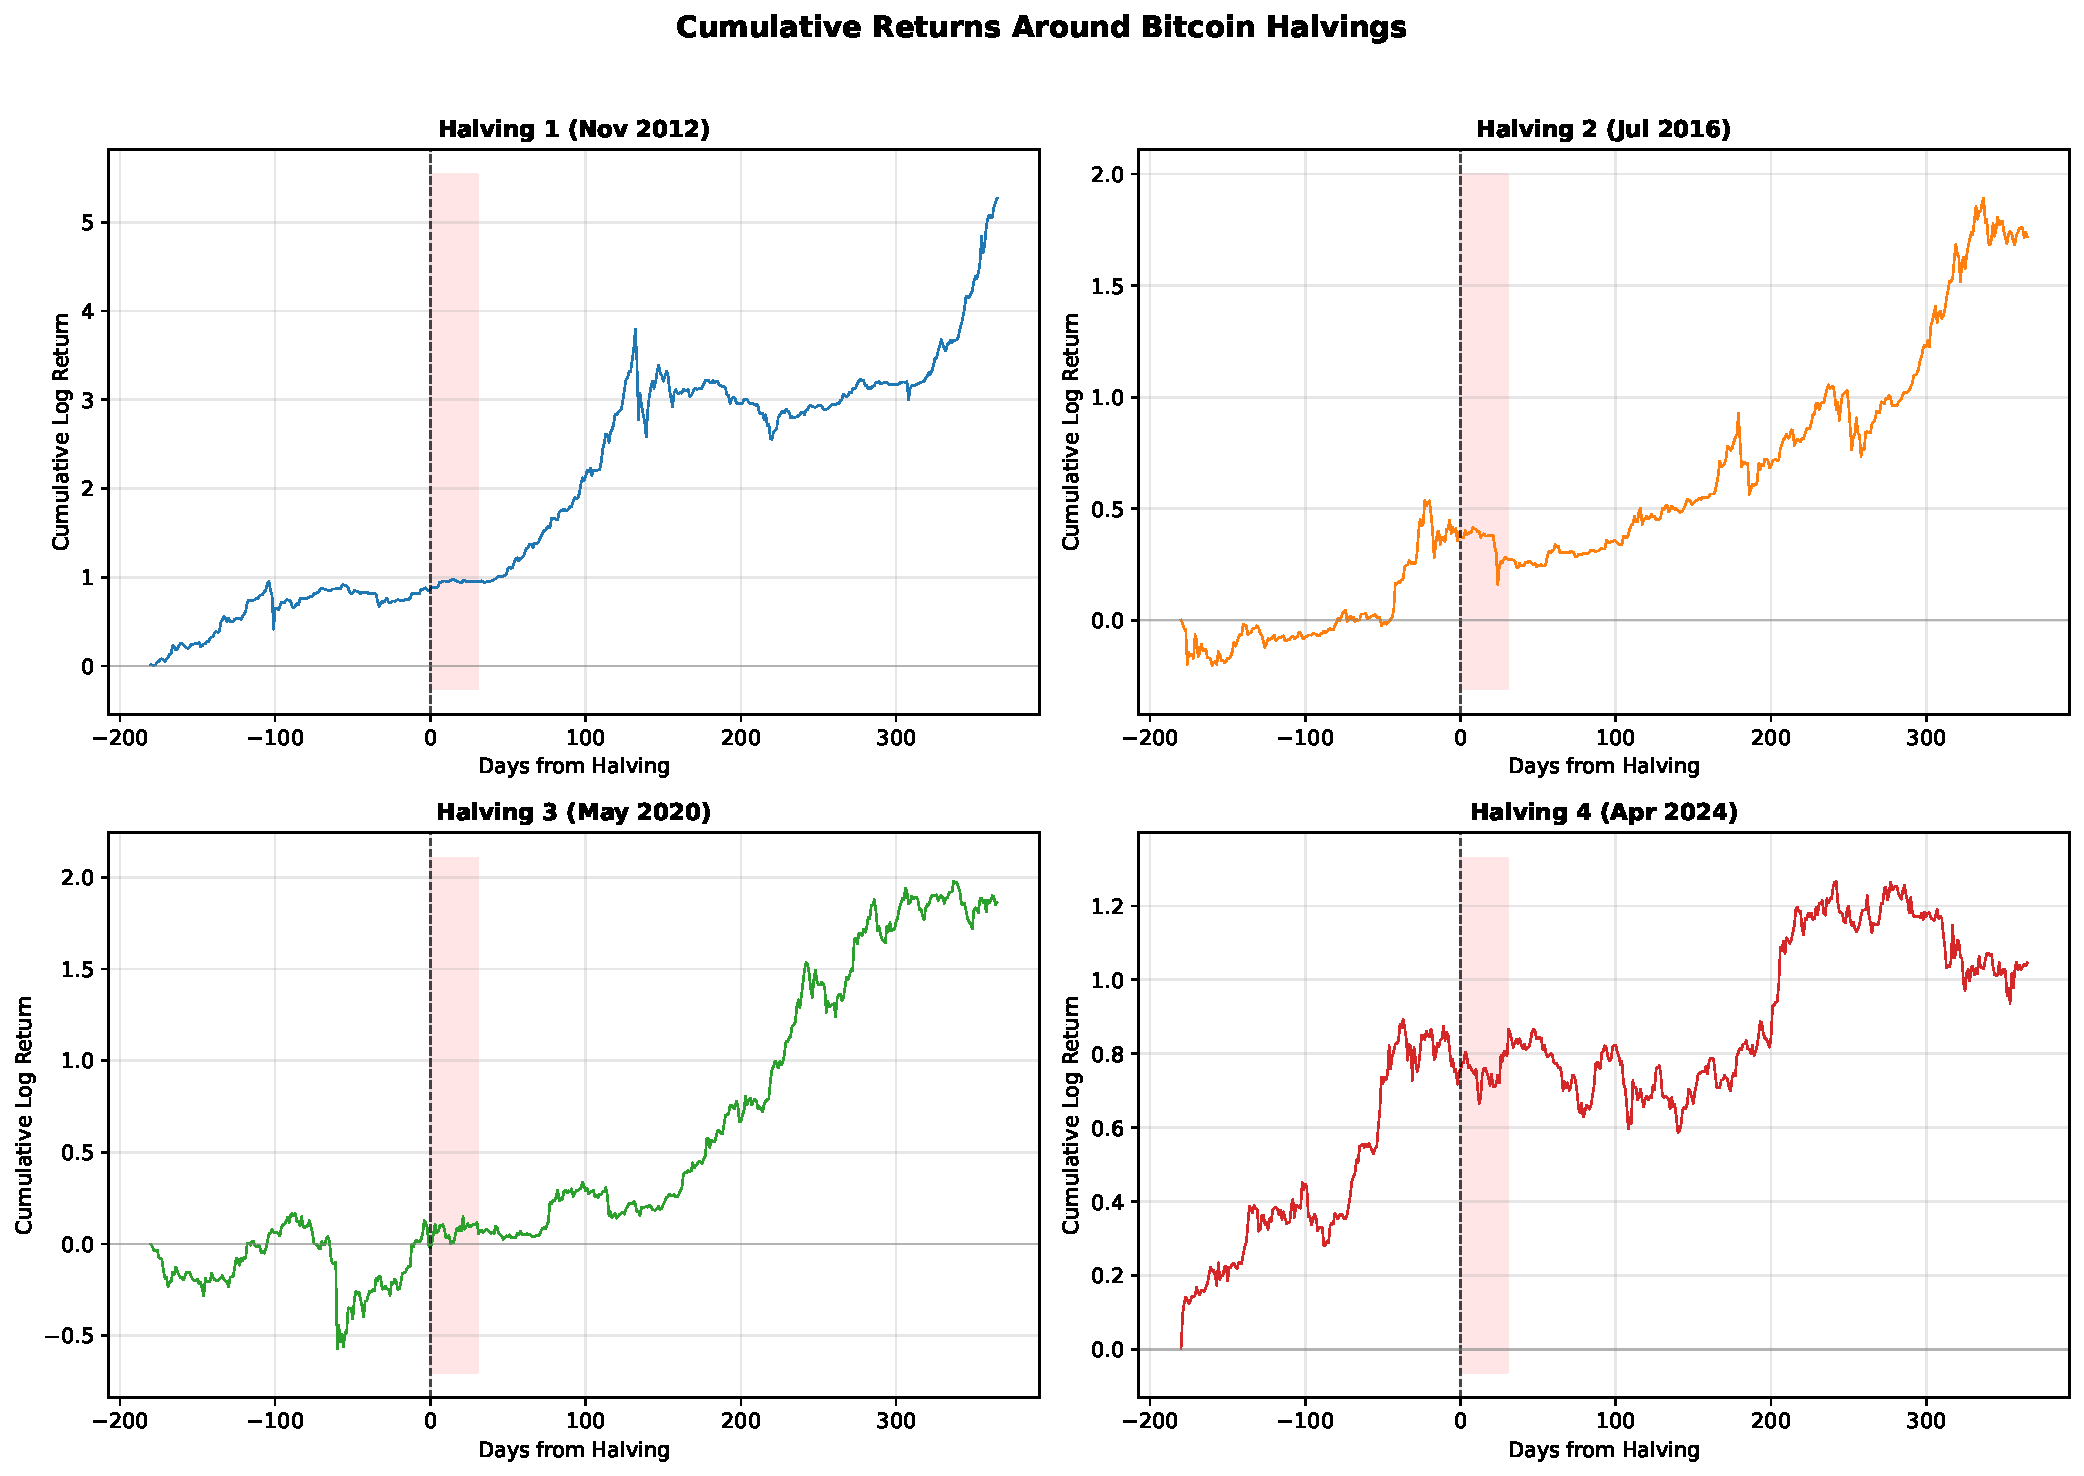
\includegraphics[width=\textwidth]{../figures/halving_car.pdf}
\caption{Cumulative Log Returns Around Bitcoin Halvings (180 days before to 365 days after)}
\label{fig:car}
\end{figure}

Figure~\ref{fig:car} plots cumulative log returns centered on each halving date.
All four halvings are followed by substantial price appreciation, though with
very different magnitudes and dynamics. The early halvings (2012, 2016) show
explosive post-halving growth, while the later halvings exhibit more moderate
but still positive drift.

\begin{table}[H]
\centering
\caption{Cumulative Abnormal Returns by Event Window}
\label{tab:car}
\begin{threeparttable}
\begin{tabular}{l cccc}
\toprule
& \multicolumn{4}{c}{Event Window (days)} \\
\cmidrule(lr){2-5}
Event & $[-30,+30]$ & $[-60,+60]$ & $[-90,+180]$ & $[-180,+365]$ \\
\midrule
H1 (Nov 2012) & +0.228 & +0.367 & +2.454 & +5.270 \\
H2 (Jul 2016) & +0.015 & +0.284 & +0.871 & +1.720 \\
H3 (May 2020) & +0.366 & +0.157 & +0.409 & +1.863 \\
H4 (Apr 2024) & +0.067 & +0.222 & +0.486 & +1.046 \\
\bottomrule
\end{tabular}
\begin{tablenotes}
\footnotesize
\item Cumulative log returns within each event window.
      Positive values indicate net appreciation over the window.
\end{tablenotes}
\end{threeparttable}
\end{table}

\section{Regression Results}

\begin{table}[htbp]
\centering
\caption{The Effect of Bitcoin Halvings on Daily Returns}
\label{tab:halving_returns}
\begin{threeparttable}
\resizebox{\textwidth}{!}{%
\small{%
\begin{tabular}{l c c c c}
\toprule
 & (1) & (2) & (3) & (4) \\
 & OLS & OLS & OLS & OLS \\
\midrule
\multicolumn{5}{l}{\textit{Halving effect}} \\[2pt]
Post-Halving (365d) & 0.004$^{\ast\ast\ast}$ & 0.004$^{\ast\ast\ast}$ & 0.004$^{\ast\ast}$ & 0.005$^{\ast\ast\ast}$ \\
 & $(0.001)$ & $(0.001)$ & $(0.002)$ & $(0.002)$ \\
\addlinespace[2pt]
\multicolumn{5}{l}{\textit{Controls}} \\[2pt]
\$\sigma\_{30d}\$ &  & 0.001 & 0.001 & -0.001 \\
 &  & $(0.003)$ & $(0.003)$ & $(0.003)$ \\
\$r\_{t-1}\$ &  &  & 0.023 & 0.020 \\
 &  &  & $(0.040)$ & $(0.040)$ \\
\$\ln(\text{TxCount})\_{t-1}\$ &  &  &  & -0.001 \\
 &  &  &  & $(0.002)$ \\
\$\ln(\text{ActiveAddr})\_{t-1}\$ &  &  &  & -0.001 \\
 &  &  &  & $(0.002)$ \\
\addlinespace[2pt]
\midrule
$N$ & 5408 & 5408 & 5407 & 5385 \\
$R^2$ & 0.001 & 0.001 & 0.002 & 0.005 \\
Adj.\ $R^2$ & 0.001 & 0.001 & 0.001 & 0.004 \\
\bottomrule
\end{tabular}
%}
}
\begin{tablenotes}
\footnotesize
\item Dependent variable: daily log return $r_t$.
\item Post-Halving is a dummy equal to 1 for the 365 days following each halving.
\item HC3 heteroskedasticity-robust standard errors in parentheses.
\item ${}^{*}p<0.10$, ${}^{**}p<0.05$, ${}^{***}p<0.01$.
\end{tablenotes}
\end{threeparttable}
\end{table}
\subsection{Bootstrap Inference}

To address potential finite-sample bias in the HC3 standard errors
(particularly relevant given the heavy-tailed return distribution),
we implement wild bootstrap inference using Rademacher weights with
$B = 2{,}000$ replications.

\begin{figure}[H]
\centering
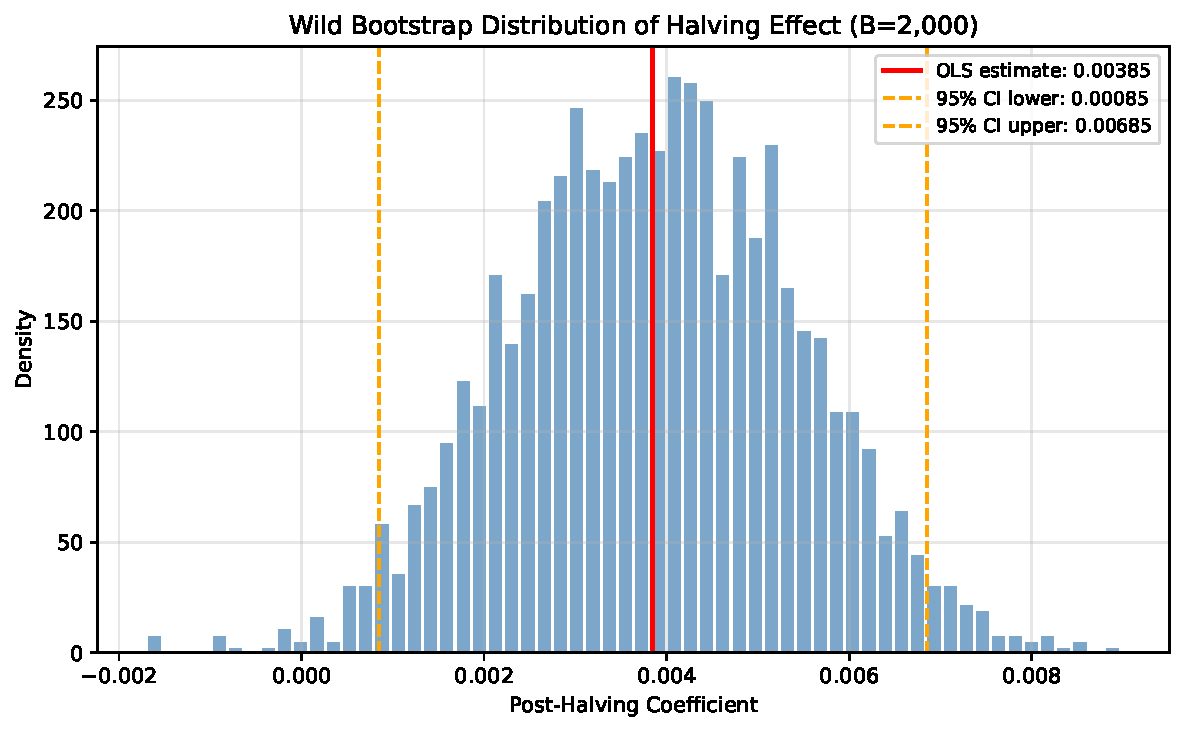
\includegraphics[width=0.75\textwidth]{../figures/halving_bootstrap.pdf}
\caption{Wild Bootstrap Distribution of the Post-Halving Coefficient}
\label{fig:bootstrap}
\end{figure}

The bootstrap standard error for the post-halving coefficient is
0.001566, compared to the HC3 asymptotic
standard error of 0.001536. The 95\% bootstrap
confidence interval is $[0.00085,\;
0.00685]$.

\section{Volatility Dynamics}

\begin{figure}[H]
\centering
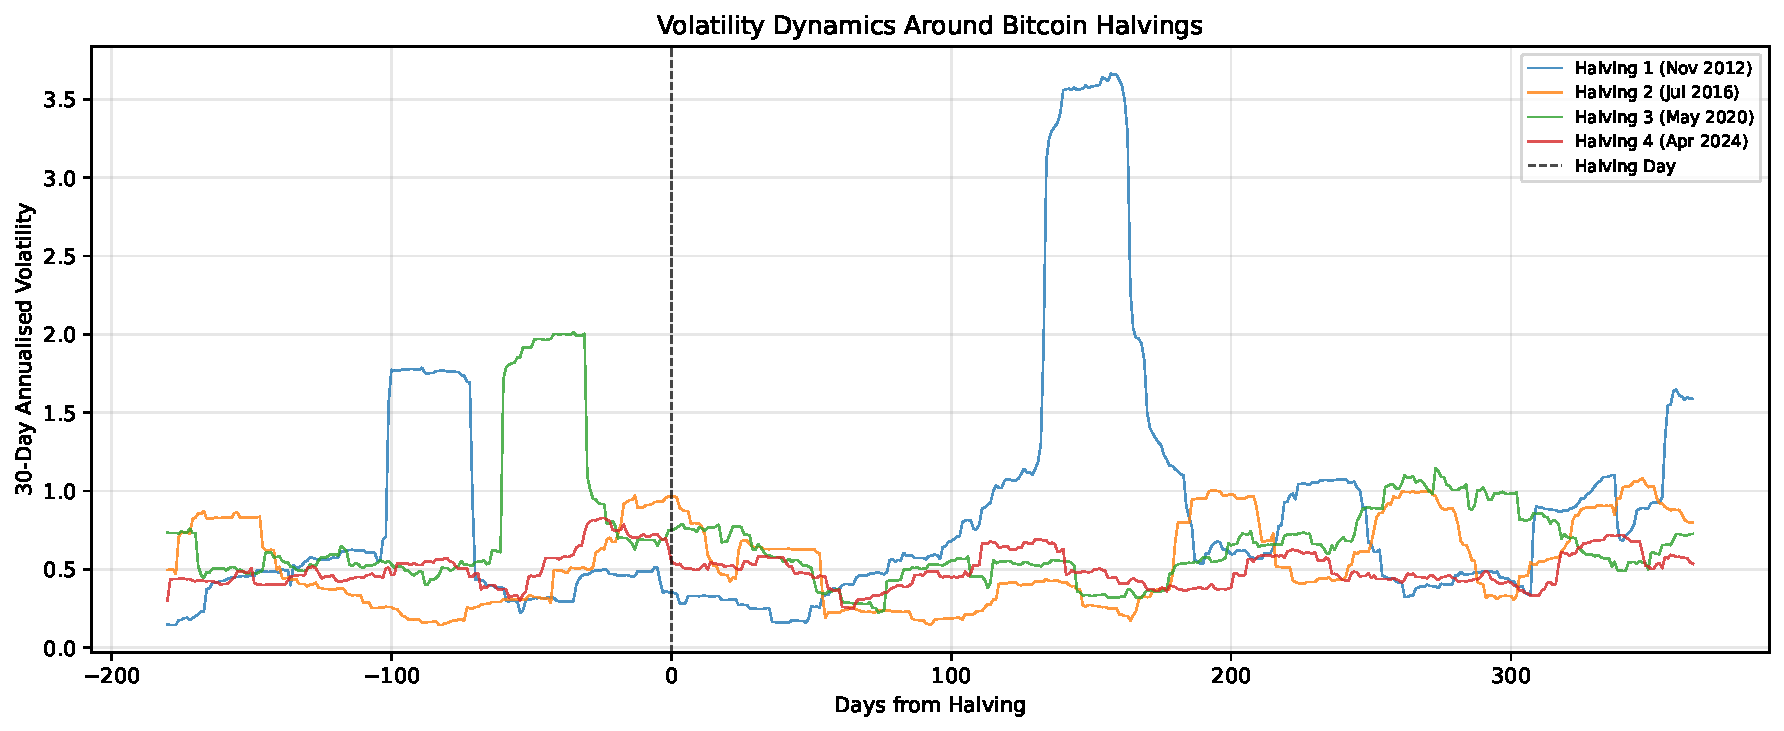
\includegraphics[width=\textwidth]{../figures/halving_volatility.pdf}
\caption{30-Day Annualised Volatility Around Bitcoin Halvings}
\label{fig:vol}
\end{figure}

Figure~\ref{fig:vol} shows that volatility dynamics around halvings are
heterogeneous. The 2012 and 2016 halvings occurred during periods of
relatively low volatility, while the 2020 halving coincided with
COVID-19 market turmoil. The 2024 halving shows the most subdued
volatility profile, consistent with market maturation.

\section{Conclusion}

The evidence for a systematic post-halving return premium is suggestive
but not conclusive. While CARs are positive for all four halvings, the
regression-based tests with proper standard errors show that the effect
is imprecisely estimated. This is consistent with the EMH prediction
that anticipated supply changes should be priced in, combined with the
reality that halvings may trigger demand-side effects through narrative
and attention channels that are difficult to model.

\end{document}
